\section{Related Work}
\label{sec:related}

% A increasingly large body of work has focused on the problem of key grouping (or Group By). There are two categories of GroupBy implementations in general, sort-based grouping and hash-based grouping. Each of these algorithms can be used for anywhere in database query related to grouping (Group By, SUM, AVE, etc) \cite{Hellerstein1996Query}.
This section provides some backgrounds on existing key grouping approaches and reviews the count-min sketch that will be used in our algorithm.
%Section A introduces the merge-sort grouping algorithm and Section B provides a detailed description on memory-constraint hash algorithm for SQL Hash GroupBy clause,  Section C and D introduces the power-law distributions  and the count-min sketch.

\subsection{Commonly Used Grouping Implementations}%2.1

\Paragraph{Merge-Sort Grouping} One of the most widely used grouping algorithm is merge-sort grouping, which is widely used in MapReduce \cite{dean2008mapreduce} and SQL Group By operator \cite{nasir2015power},\cite{mysql2009mysql},\cite{boicea2012mongodb},\cite{momjian2001postgresql},\cite{agrawal2005database}. The Hadoop MapReduce uses a merge-sort at both the Map and Reduce phases to group kv-pairs. These kv-pairs to be grouped will be constantly written to the memory buffer. The buffer is used to collect kv-pairs in batches, so as to minimize the impact of disk I/O. The entire buffer size is limited. As the amount of data in the buffer reaches the threshold, a background spilled thread sorts these kv-pairs in the memory buffer in accordance with the key, and writes these kv-pairs that have been sorted in the buffer to disk as a partial sorted file. Each spilling operation generates a spilled file on disk. Finally, a merge phase is required to sort these partial sorted files to generate the final sorted file (i.e., the data in the file are grouped). Merge-sort can achieve the purpose of aggregating kv-pairs for any amount of data, which is highly scalable. However, keeping different groups in order is unnecessary because the aim is making the kv-pairs that are in the same key continuously stored on disk. Therefore, merge-sort grouping will result in unnecessary computational overhead.


%In SQL database, The default Group By implementation is to scan the entire table, e.g. group records in table by merge-sort algorithm or make use of index based on columns specified by Group By clause to avoid sorting again \cite{mysql2009mysql}. Sorting is never  the  best, except  when  tables  are ordered  in  advance  or  when the  result  have  to  be sorted  on operation  key \cite{Bratbergsengen1984Hashing}.


%However, the execution efficiency is not high enough. The merge-sort algorithm aggregates kv-pairs with the same key by sorting key completely, so that the grouping keys are ordered among different groups. Commonly, keeping different groups in order is redundant because the aim of grouping is to store kv-pairs having the same key on adjacent locations on the disk, and it��s irrelevant Whether grouping keys are sorted between two groups. Therefore, merge-sort for aggregating kv-pairs will result in unnecessary computational overhead. on the other hand, the amount of memory required for sorting is proportional to the total number of kv-pairs in the buffer rather than the number of distinct keys.


\Paragraph{Memory-Constraint Hash Grouping}%2.2
Some SQL databases (e.g., MariaDB) that use a hash grouping aggregation strategy for GroupBy operations \cite{bartholomew2012mariadb}. We refer to this approach as \emph{memory-constraint hash grouping}.  The memory-constraint hash is similar to hash join, it does not require sort but more memory. \textcolor{red}{Memory-constraint hash partitions the large task  into smaller subtasks  where the subtasks can be executed in memory completely \cite{Bratbergsengen1984Hashing},\cite{HashAggregate15}. If the size of data to be grouped exceeds the memory limit, one or more buckets will be spilled to disk. Then the records that are hashed to the spilled buckets will be divided up into the corresponding partitions in disk. Once all input groups have been processed, the completed in-memory groups will be output and repeat the algorithm by reading back and aggregating one spilled partition at a time. However, when processing data sets whose group sizes follow power-law distributions, the sub-tables sizes are not balanced, which leads to multiple recursive partitions and downgrade grouping performance.}

%including any partial aggregated results along with any additional new rows that will be hashed to the spilled buckets or partitions


\subsection{Group Size Distribution}
%Many of the things that scientists measure have a typical size or ``scale'' --- a typical value around which individual measurements are centred. But not all things we measure are peaked around a typical value, some vary over an enormous dynamic range \cite{MEJPower}, those things following the power-law distributions are like this.

% \textcolor{red}{should be rewrite, please refer to PowerGraph paper. The goal is to tell readers the group sizes are indeed following powerlaw distribution. Besides the figure, you might want to show some numbers, like 99\% data are from top 10\% big groups, or some thing like that. You might also want to say some thing that for the extremely large groups, the traditional grouping tech will not work. and say why}

Power-law distributions \cite{MEJPower} occur in an extraordinarily diverse range of phenomena, e.g., the frequency of use of words in any human language \cite{George1949Human}, the number of hits on web pages \cite{Adamic2000The}. As shown in Figure \ref{fig: distributions}, the group sizes in four data sets(see Sec. \ref{sec:experiment} for dataset description) are also follow the power-law distributions and vary over an enormous dynamic range. The distributions are all right-skewed, it means that a bulk of groups occurs for fairly small sizes and only a small number of groups are much higher, in more detail, about 80\% data are from top 20\% big groups in Twitter, web-BerkStan and Google, the top 20\% big groups occupy about 90\% size in Pareto.

For some extremely large groups whose sizes are larger than the available memory, when the groups are processed by some traditional grouping approaches, the endless recursive reading from and writing to disk may occur, and then these approaches can not work.



\begin{figure}[t]%figure 2
\begin{center}
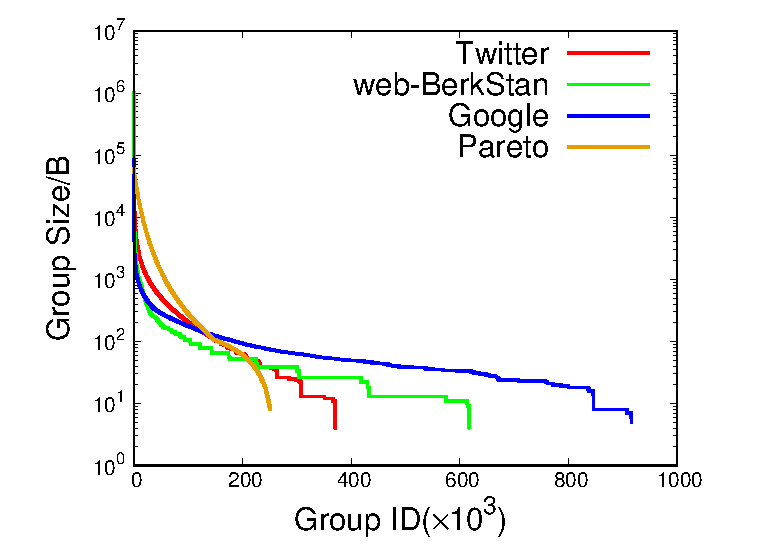
\includegraphics[width = 2.8in]{fig/distributions.eps}
%\includegraphics[width=.5\textwidth]{fig/pareto_index_hash}
\caption{The group size distributions for different data sets.}
\label{fig: distributions}
\end{center}
\end{figure}


%Based on the right-skew property of power-law distributions in reality, Pareto principle(also known as 80/20 rule)\cite{Box1986An}, \cite{MEJPower} is proposed, it is is borne out by more detailed observations of the wealth distribution. It states that about 80\% of the wealth should be in the hands of the richest 20\% of the population(the so-called ``80/20 rule''). According to the Pareto principle, we can get that roughly 80\% of the effects come from 20\% of the causes for many events. Mathematically, the 80/20 rule is roughly followed by a power-law distribution for a particular set of parameters. Besides the wealth distribution, the Pareto principle can be applied to optimization efforts in computer science, engineering control\cite{Gen2000Network} and many other applications.

%For a data set whose group sizes follow a power-law distribution, we can distinguish between the big groups and small groups roughly on the basis the Pareto principle, the ratio between big groups and small groups obeys the 80/20 rule.
%We extract the groups that are the top 20\% in size from four data sets, these big groups occupy about 80\% of the data sets as shown in Table \ref{tab:percentage}.

\begin{comment}
\begin{table}
  \caption{Percentage of the size of the big groups}
  \label{tab:percentage}
  \begin{tabular}{cccc}
    \toprule
    dataset & total size & big group size & percentage\\
    \midrule
    Twitter & 180.4MB & 142MB & 78\%\\	
	web-BerkStan & 102.5MB & 80.0MB &78\%\\
	Google & 97.2MB & 61M & 63\%
	Pareto  & 575.4MB & 519MB & 90\%\\
    \bottomrule
  \end{tabular}
\end{table}
\end{comment}


\subsection{The Count-Min Sketch}

The count-min sketch (CM sketch)\cite{Cormode2009Count},\cite{10.1007/978-3-540-24698-5_7} is a probabilistic data structure that serves as a frequency table of events in a data stream, it uses hash functions to map events to frequencies at the expense of overcounting some events due to collisions.

A CM sketch is represented by a two-dimensional array counting with width $w$ and depth $d$. Additionally, $d$ hash functions $h_{1} ...h_{d}$ are chosen uniformly at random from a pairwise-independent family. The space used by Count-Min sketches is the two-dimensional array and $d$ hash functions. The CM sketch is simple to construct and counting the frequencies of the unique items in data stream quickly.

%\textcolor{red}{the following paragraphs should be rewriten, what is $h_{j}$ ?  Also, please give more intuitions.}

%\emph{Data Structure}: A CM sketch is represented by a two-dimensional array counts with width $w$ and depth $d$. If the error of group sizes is within a factor of $ \varepsilon $ with probability $ \delta$, the depth $d$ is $\lceil ln(1/\delta) \rceil $, the width $w$ is $\lceil e/\varepsilon\rceil $. Each entry of the array is initially zero. Additionally, $d$ hash functions $h_{1} ...h_{d}$ are chosen uniformly at random from a pairwise-independent family.

The count-min sketch is named after the two basic operations, counting first and computing the minimum next. When it gets an item $a_{i}$ with a quantity of $c_{i}$ , then $c_{i}$ is added to one count in each row; the counter is determined by the $d$ hash function. Formally, set $\forall 1 \leq j \leq d: count[j,h_{j}(a_{i})]\leftarrow count[j,h_{j}(a_{i})] + c_{i}$. After counting the frequency roughly, the frequency of a unique item $a_{i}$ is the minimum of statistical results in each row, for $\forall 1 \leq j \leq d$, it is given by $f_{i} = min_{j}count[j,h_{j}(a_{i})]$.

On the other hand, each row of the CM sketch can reflect the distribution of group sizes, this property can help us distinguish the big groups and small groups with avoiding large-scale sorting.

%In our algorithm, the CM sketch will be used to counting the group sizes in the data sets, the distinction between big groups and small groups is based on these rough group sizes. When calculating the group sizes, the CM sketch has the two basic operations: counting first and computing the minimum next.
%We first traverse the input data set to be grouped, When getting a $\langle key, value\rangle$ pair, the group that this kv-pair belongs to can beobtained by its unique $key$, the group size will be updated by the kv-pair size $sizeof(key)$+ $sizeof(value)$, then $sizeof(kv)$ are added to one count in each row; the counter is determined by the hash functions. Formally, set $\forall 1 \leq j \leq d: count[j,h_{j}(key)]\leftarrow count[j,h_{j}(key)] + sizeof(key) + sizeof(value)$. After counting, the size to a group with $key$ is given by $f_{key} = min_{j}count[j,h_{j}(key)]$.

Our strategy is to leverage the CM sketch to counting the group sizes in the data set roughly, the rough group sizes are used to distinguish between the big groups and small groups depending on Pareto principle. Then the big groups and small groups are processed separately, the big groups are grouped by the indexing-filling method to reduce the I/O cost, the small groups are processed by partitioned hash grouping approach. PowerHash can finish the key grouping operation in limited memory with high efficiency.
